\begin{figure}[t]
    \centering
    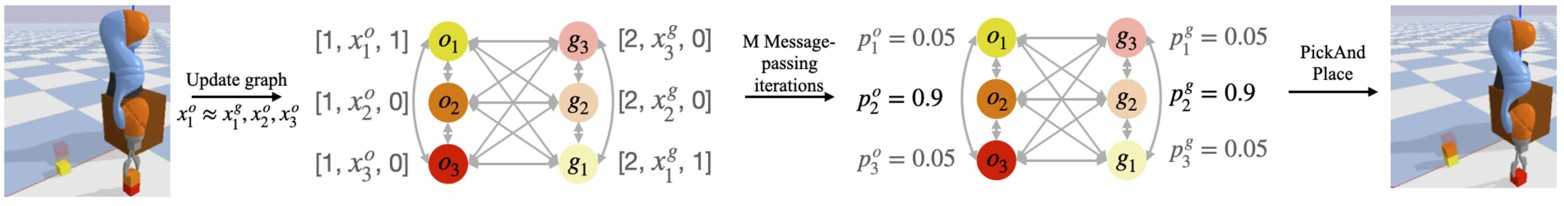
\includegraphics[width=1\textwidth]{figures/images/ch4/geometric_graph_computation.jpg}
    \caption{Computation flow in a scene represented by a Geometric Graph. Object nodes ($o_{i}$) and goal nodes ($g_{i}$) are created, with edges connecting them based on spatial and semantic relationships. A GNN classifies the nodes, selecting one object node and one goal node. These nodes are then passed as input to a motion primitive, which generates the necessary actions to move the selected object towards the target goal.}
    \label{fig:geometric_graph_computation}
\end{figure}
